\chapter{系统测试}
在实现系统功能的基础上,需要对系统的功能、性能进行测试。本文搭建了多节点云平台,在此基础上进行了功能测试和性能测试。功能测试验证了租户虚拟网络之间的隔离性,带宽、时延的测量功能,以及租户数据传输的链路切换功能。性能测试对SDN模式下流表的下发性能进行测试,验证SDN模式下集群大小对流表下发性能的影响。通过对SDN模式和传统模式下数据传输效率的测试。验证SDN模式下数据传输的效率是否有所降低。
\section{实验环境}
本文搭建的基于SDN的云平台,包含4台物理服务器,其中有一台单独配置为网络节点,主要负责云平台中网络资源的管理。两台单独配置为计算节点,一台配置为控制节点和计算节点。计算节点主要负责虚拟机的创建,控制节点实现集中调度的功能。具体各节点以及服务器硬件信息如表\ref{table:environment}所示。

\begin{table}[!htb]
    \centering
	\caption{云平台实验环境}
	\label{table:environment}
	\begin{tabular}{|c|c|c|}
	\hline 
	属性 & 服务器配置 & 操作系统 \\
	\hline
	计算节点& \enter{ubuntu1(内存:64G,CPU:24核,硬盘:2.3T) \\ubuntu5(内存:64G,CPU:24核,硬盘:2.4T)\\ ubuntu6(内存64G:,CPU:24核,硬盘:450G)} & Ubuntu-14.04 \\
	\hline
	网络节点 & ubuntu-1404-1(内存:24G,CPU:4核,硬盘:1.4T) & Ubuntu-14.04 \\
	\hline
	控制节点 & ubuntu5(内存:64G,CPU:24核,硬盘:2.4T) & Ubuntu-14.04 \\
	\hline
	\end{tabular}
\end{table}

在云平台中,本文选用project-likai租户进行相关测试。该租户共计包含11台虚拟机,其中10台虚拟机基于CirrOS镜像进行创建,1台虚拟机基于Ryu镜像进行创建,该镜像集成Ryu控制器,同时为该镜像添加了开机自启动脚本,在虚拟机启动时,自动运行Ryu控制器及相关应用。默认情况下,该控制器占用TCP的6633端口,租户可以登录该控制器虚拟机,自定义控制器的启动端口。虚拟机的详细列表如图\ref{fig:allhosts}所示,图中详细介绍了虚拟机的名字、镜像、IP地址、虚拟机的运行状态,以及虚拟机的配置信息。图中的m1.tiny,代表的配置信息为内存512M、硬盘1G、vCPU为1核。

\begin{figure}[!htb]
  \centering
  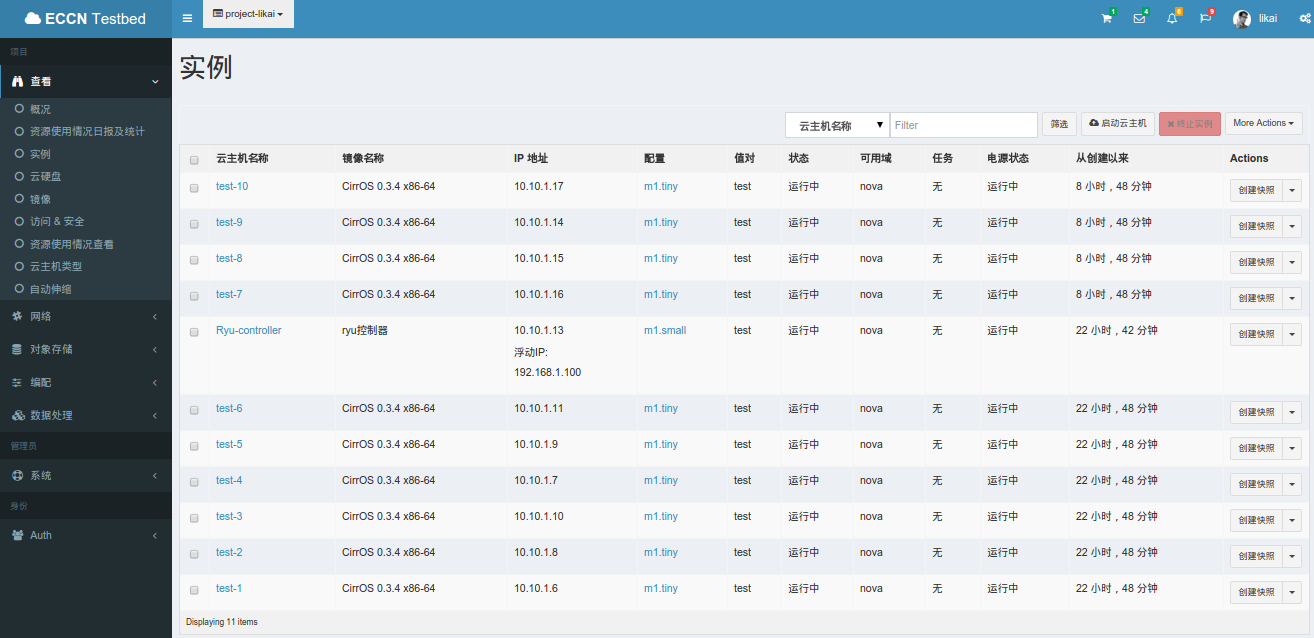
\includegraphics[width=0.8\textwidth]{logo/allhosts.png}
  \caption{租户虚拟机列表}
  \label{fig:allhosts}
\end{figure}
\section{功能测试}
\subsection{租户隔离性}
本文基于底层的物理网络,进行了虚拟网络的创建,具体如图\ref{fig:create-virtual}所示,由图中可以看出,本文选取test-3,test-4,switch0,switch2,switch3,switch5,switch7进行虚拟网络的创建,控制器运行在Ryu-controller虚拟机中,IP地址为192.168.1.100,租户创建的虚拟网络由运行在该虚拟机中的Ryu控制器进行集中管控。

\begin{figure}[!htb]
  \centering
  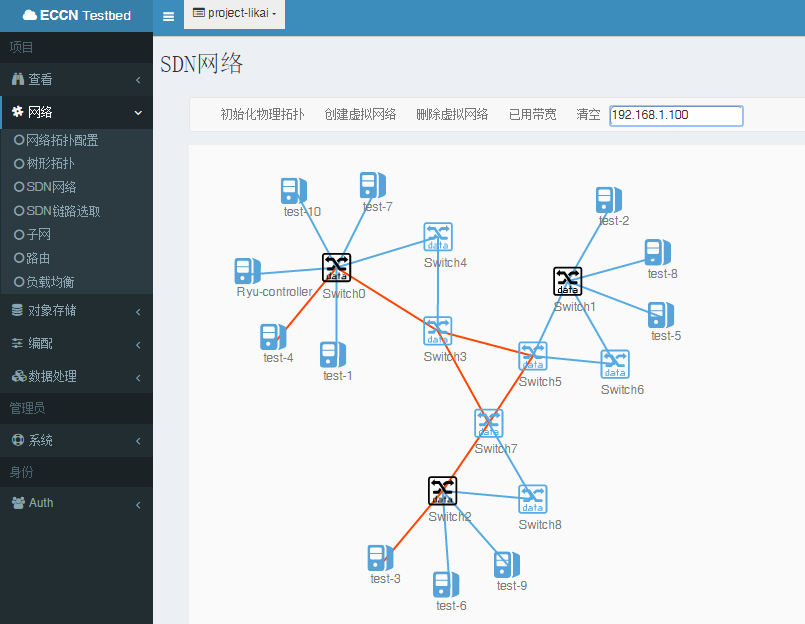
\includegraphics[width=0.8\textwidth,height=0.50\textwidth]{logo/create-virtual.png}
  \caption{虚拟网络创建图}
  \label{fig:create-virtual}
\end{figure}

创建生成的虚拟网络如图\ref{fig:virtualnet-test}所示,图中的交换机和虚拟机与上图之间是一一对应的关系。

\begin{figure}[!htb]
  \centering
  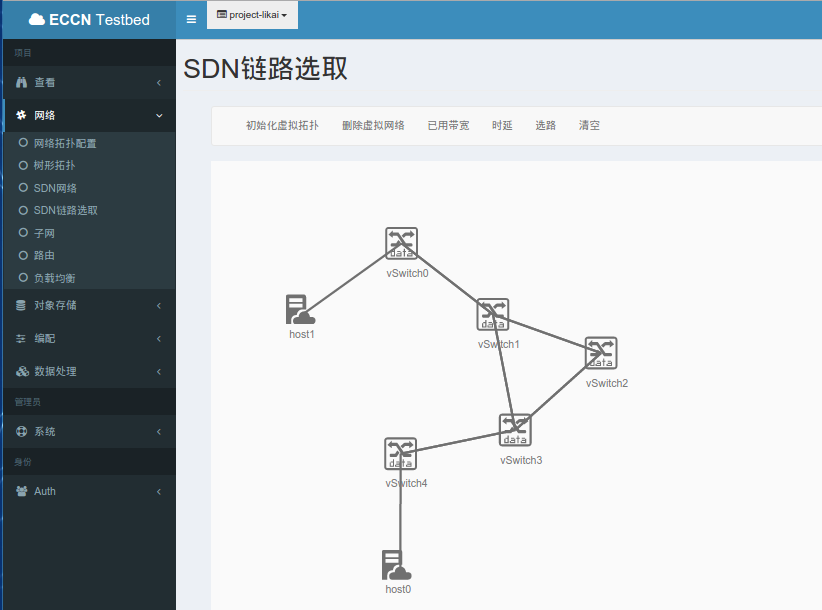
\includegraphics[width=0.8\textwidth,height=0.50\textwidth]{logo/virtualnet.png}
  \caption{虚拟网络拓扑图}
  \label{fig:virtualnet-test}
\end{figure}

为了进行租户隔离性的测试,本文选取test-3虚拟机,让其分别与test-4和test-5进行ping测试,由图\ref{fig:subfig:a}可以看出,test-3与test-4属于同一个虚拟网络,可以进行正常通信。而对于test-3和test-5,由图\ref{fig:subfig:b}可以看出,两虚拟机不属于租户创建的同一个虚拟网络内,故不能直接进行通信。实验表明,租户创建的虚拟网络之间是相互隔离的,数据传输是安全可靠的。

\begin{figure}[!htb]
 \centering
 \subfigure[test-3与test-4测试结果]{
   \label{fig:subfig:a} %% label for first subfigure
   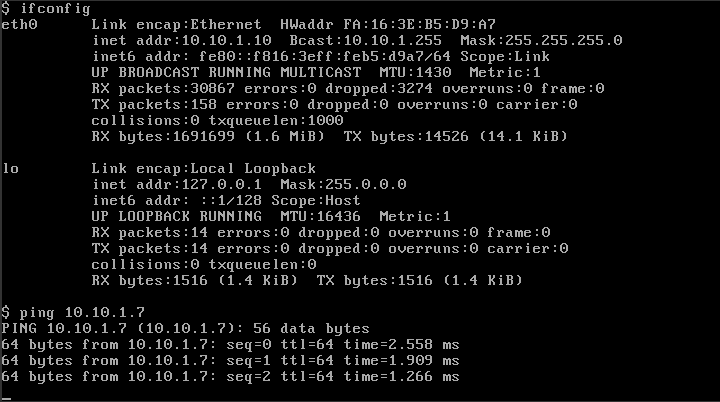
\includegraphics[width=0.485\textwidth]{logo/ping.png}}
 %\hspace{1in}
 \subfigure[test-3与test-5测试结果]{
   \label{fig:subfig:b} %% label for second subfigure
   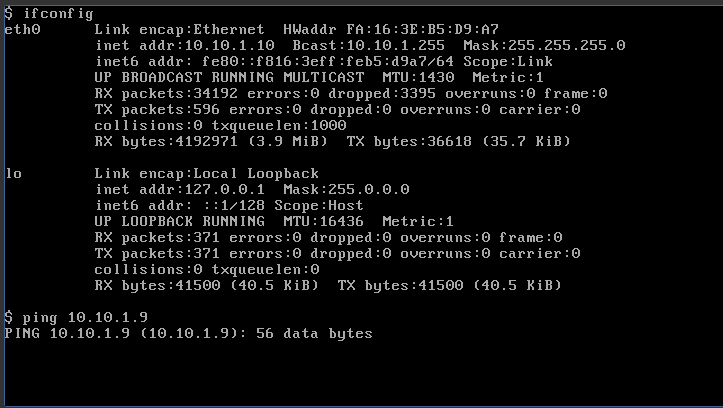
\includegraphics[width=0.48\textwidth]{logo/ping-cannot.png}}
 \caption{租户隔离性测试图}
 \label{fig:isolation} %% label for entire figure
\end{figure}
\subsection{带宽、时延测量}
为方便租户在前端进行网络负载的查看,本文实现了对物理网络和虚拟网络带宽、时延的测量以及前端界面的可视化。对于物理网络的带宽测量,测试结果如图\ref{fig:bandwidth}所示,实验表明,租户可以查看到物理网络当前的带宽使用情况。

\begin{figure}[!htb]
  \centering
  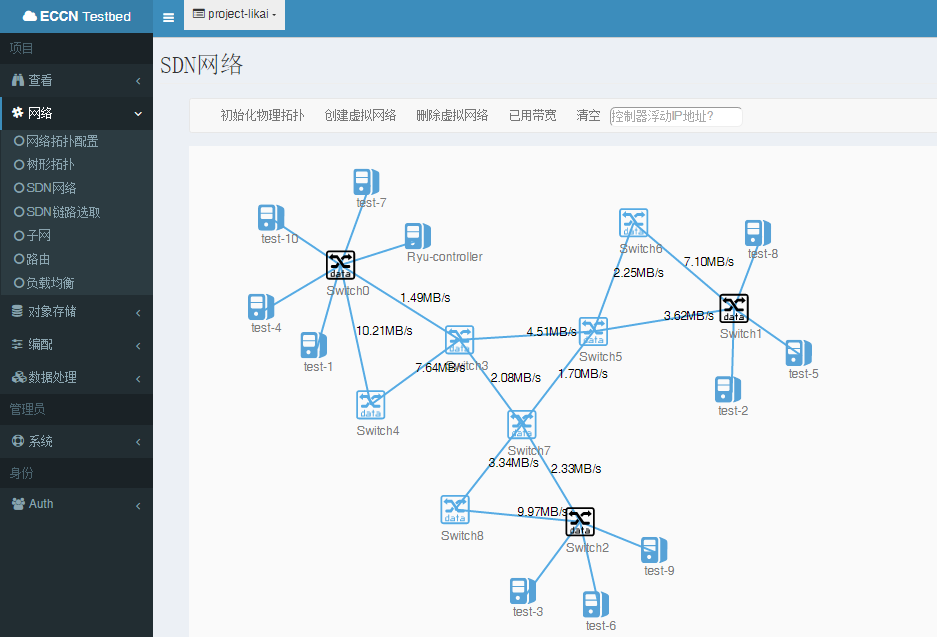
\includegraphics[width=0.8\textwidth,height=0.50\textwidth]{logo/bandwidth.png}
  \caption{物理网络带宽测量图}
  \label{fig:bandwidth}
\end{figure}

对于时延,本文仅仅实现了对虚拟网络的时延测量工作,通过为租户控制器开发的北向应用,实现虚拟网络的时延测量工作,测试结果如图\ref{fig:virtualdelay}所示,实验表明,租户控制器可以实现对虚拟网络时延数据的测量工作。

\begin{figure}[!htb]
  \centering
  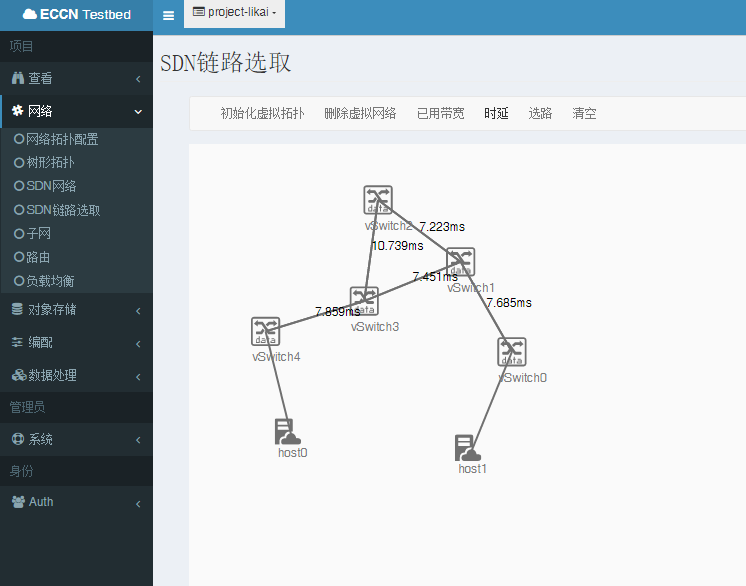
\includegraphics[width=0.8\textwidth,height=0.50\textwidth]{logo/virtualdelay.png}
  \caption{虚拟网络时延测量图}
  \label{fig:virtualdelay}
\end{figure}
\subsection{链路切换}
对于租户创建的虚拟网络,本文实现了链路切换的功能,可以让租户实现对数据传输路径的定制化,如图\ref{fig:virtualnet-test}所示,host0和host1之间有存在两条传输路径。分别为链路1:host1-vswitch0-vswitch1-vswitch3-vswitch4-host0,和链路2:host1-vswitch0-vswitch1-vswitch2-vswitch3-vswitch4-host0,本文首先选取链路1进行数据传输,通过选路按键,进行定制化流表下发后,host0与host1进行ping测试,得到的带宽测量图如图\ref{fig:subfig-virtual:a}所示,由图中可以看出,该模式下,数据按照链路1进行数据传输。随后,选取链路2,并通过选路下发定制化流表,进而进行带宽测试,发现数据传输的通路已然变为链路2,具体如图\ref{fig:subfig-virtual:b}所示。实验表明,租户可以自定制数据转发路径,通过选路操作进行定制化流表的下发,从而实现对数据转发路径的控制操作。

\begin{figure}[!htb]
 \centering
 \subfigure[定制化链路1]{
   \label{fig:subfig-virtual:a} %% label for first subfigure
   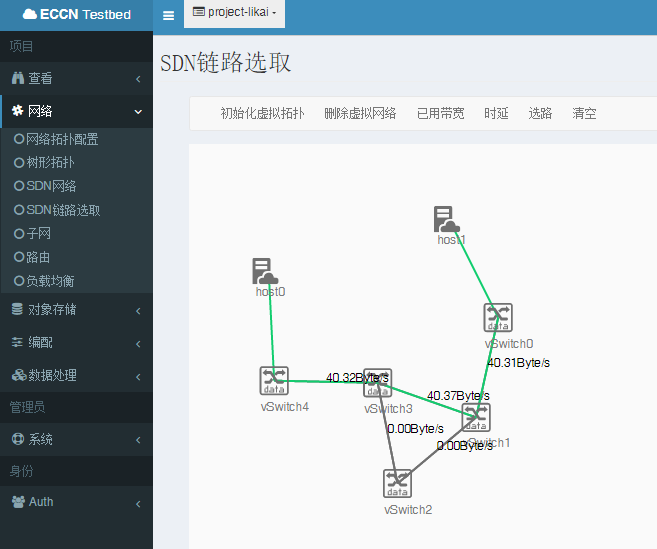
\includegraphics[width=0.48\textwidth,height=0.40\textwidth]{logo/band-virtual.png}}
 %\hspace{1in}
 \subfigure[定制化链路2]{
   \label{fig:subfig-virtual:b} %% label for second subfigure
   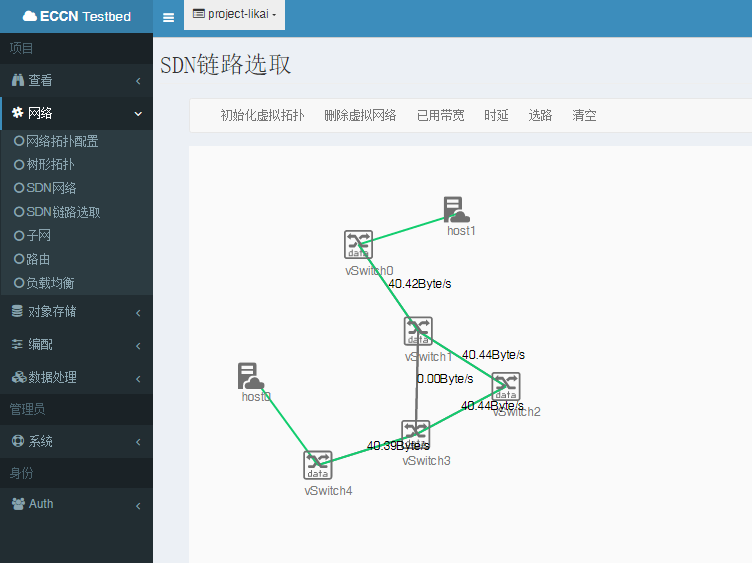
\includegraphics[width=0.48\textwidth,height=0.40\textwidth]{logo/band-virtual-2.png}}
 \caption{虚拟网络链路切换图}
 \label{fig:customlink} %% label for entire figure
\end{figure}
\section{性能测试}
\subsection{流表下发性能测试}
引入SDN后,在SDN模式下,对单条流表的下发时间做了测试,验证随着数据中心网络的扩大,流表的下发效率是否会急剧下降,对数据的传输是否有较大的影响,本文分别对租户A和租户B的网络进行了测试。测试结果如图\ref{fig:flow-time}所示。结果表明,随着云数据中心网络的扩大,单条流表的下发时间随之增长,但增长的趋势逐渐变缓,效率并未大幅下降,仍能满足用户对数据传输效率的要求。

\begin{figure}[!htb]
  \centering
  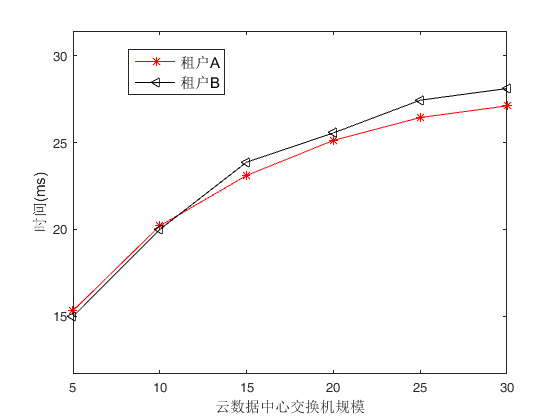
\includegraphics[width=0.6\textwidth,height=0.40\textwidth]{logo/flow-time}
  \caption{数据中心单条流表下发时间}
  \label{fig:flow-time}
\end{figure}
\subsection{数据传输效率测试}
本文分别对SDN架构和传统OpenStack架构下的数据传输进行测试,对比引入SDN后,数据的传输速率是否受到了影响。本文以租户A的网络作为实验对象,在其中的两台虚拟机之间传输固定大小的数据包,分别测试在传统架构和SDN架构下的数据传输时间,数据包的大小在200MB-600MB之间,实验结果如图\ref{fig:transmission}所示,结果表明,引入SDN架构后,数据的传输速率并未得到大幅下降,仍能很好的满足用户的需求。
\begin{figure}[!htb]
  \centering
  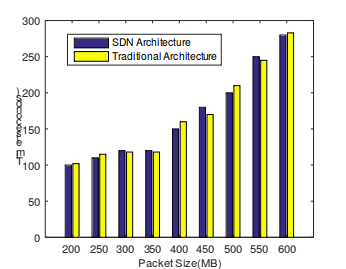
\includegraphics[width=0.6\textwidth,height=0.40\textwidth]{logo/transmission}
  \caption{SDN与传统架构下的平均数据传输效率}
  \label{fig:transmission}
\end{figure}
\section{本章小结}
本章主要是对系统进行了测试,首先介绍了实验环境,对云平台的服务器信息做了简单概述。测试主要分功能和性能测试,功能测试主要对租户的隔离性,链路带宽、时延的测量,以及链路切换进行了验证。性能测试主要包括流表的下发效率以及SDN模式与传统模式数据传输效率。结果表明,SDN模式并未降低数据传输效率,能够很好的满足用户的需求。